\documentclass[12pt,a4paper]{report}
%\begin{usepackages}
\usepackage[dutch]{babel}
\usepackage{graphicx}
\usepackage{url}
\usepackage{hyperref}
\usepackage{fancyhdr}
\pagestyle{fancy}
\usepackage{float}
\usepackage{lastpage}
\usepackage{cite}
\usepackage{makeidx}
\makeindex
\usepackage{hyperref}
%\end{}

\begin{document}
%\begin{headers en footers}
\lhead{\leftmark}
\chead{}
\rhead{}
\lfoot{Ward Pennemans}
\cfoot{\thepage \hspace*{1pt} / \pageref{LastPage}}
\rfoot{2011-2012 / 2TinH}
%\end{}
%\begin{titelpagina}
\begin{figure}
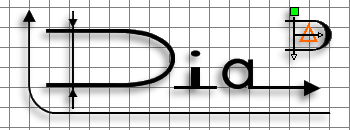
\includegraphics[scale=1]{images/dia.png}
\vspace{-100pt} 
\end{figure}
\title{DIA}
\author{Ward Pennemans - 2TinH}
\maketitle
\thispagestyle{empty}
%\end{}

\begin{flushleft}
%-----introductie-----
Dit document is geschreven met behulp van \LaTeX{}\index{Latex}. Dit is een reeks makro's ontworpen door Leslei Lamport in 1994. Het is een pakket dat gebruik maakt van de "programmeercode" \TeX{}\index{Tex}, ontworpen in 1984 door Donald E. Knuth voor het uitzetten van wiskundige teksten en formules. Het is te vergelijken met HTML\index{HTML}. Aangezien \LaTeX{} geen programma is moet er worden gebruik gemaakt van een applicatie om teksten te schrijven. Om deze tekst te schrijven en te compileren wordt er gebruik gemaakt van de programma's Texmaker\index{TexMaker} en MiKTeX\index{MiKTeX}.

\begin{table}[H]
\begin{tabular}{|l || l  l  l|}
\hline
gebruikt voor &&& \\
\hline
Opdracht & Dia & & \\
Document & LaTeX & TexMaker & MiKTeX\\
Versiebeheer & GIT & GITHUB & \\
MailServer & Mutt & postfix & \\
Bibliografie & BibTeX & &  \\
\hline
\end{tabular}
\centering
\caption{gebruikte hulpmiddelen voor deze opdracht}
\end{table}
%-----introductie-----

%-----Inhoud-----
\tableofcontents
%-----Inhoud-----

\chapter{Dia}
%\begin{sectie "Wat is Dia?"}
\section{Wat is Dia?}
\paragraph*{}
Dia\index{Dia} is een gratis en open source\index{Open source} applicatie om technische diagrammen te ontwikkelen, en kan objectief worden vergeleken met Visio\index{Visio} van Microsoft\index{Microsoft}. Het programma is gebaseerd op het GTK+\index{GTK+} principe. GTK+ of GIMP\index{GIMP} Toolkit is een multiplatform applicatie om gebruikersomgevingen\index{Gebruikersomgevingen} te ontwerpen. Net zoals GTK+ is Dia geschreven in de programmeertaal C\index{C(programmeertaal)}. 
\paragraph*{}
Op dit moment heeft Dia een aantal hulpmiddelen om de gewenste schema's eenvoudig te ontwerpen, nl. ERD-schema's(Entity Relationship Diagram)\index{Entity Relation Diagram (ERD)}, UML diagrammen\index{UML}, stroomdiagrammen, netwerkschema's, elektriciteitsschema's en andere. Een andere, zeer bruikbare eigenschap van Dia is dat het mogelijk is om eenvoudig bestanden op te slaan als en te openen van een XML-document\index{XML}.
Omdat dia eenvoudig en vriendelijk is in gebruik, kunnen mensen met weinig ervaring er toch eenvoudig met werken. Toch is het programma ook flexibel en krachtig genoeg om de meer ervaren gebruikers toe te laten om zeer geavanceerde schema's te ontwerpen.
\paragraph*{}
De laatste versie van Dia op dit moment is 0.97.2, beschikbaar sinds 18/12/2011. Deze versie is te downloaden op \textit{http://dia-installer.de/}.
\pagebreak
%\end{}
%\begin{sectie "Oorsprong"}
\section{Oorsprong}
\paragraph*{}
Dia is ontwikkeld door Alexander Larsson . Hij stopte met het ontwikkelen van Dia en stapte over naar GNOME\index{GNOME} en andere projecten. Ook zijn opvolger, James Henstridge ging over tot het werken met andere projecten. Hierna werden Cyrille Chepelov en Lars Raeder Clausen hoofd van ontwikkeling van Dia. Het programma wordt onderhouden door een groep van software ontwikkelaars, Dia developers\index{Dia developers}, die bestaat uit Hans Breuer, Steffen Macke en Sameer Sahasrabuddhe.
%\end{}
%\begin{sectie "Waarom Dia gebruiken?"}
\section{Waarom DIA gebruiken?}
\paragraph*{}
Dia is een open source software\index{Open source}. Hierdoor is het een zeer flexibel programma dat voldoet aan de eisen van verschillende gebruikers. Het grootste voordeel ten opzichte van concurrenten zoals Visio\index{Visio} is dat het een gratis software is. Dia maakte in de vorig versies gebruik van single document interface\index{Single Document Interface}, d.w.z. dat er voor elk schema een nieuw venster wordt geopend. Dit kan zowel positief als negatief zijn. Voor een klein aantal projecten is het eenvoudig dat elk schema een apart venster heeft met een eigen toolbar. Echter indien er tegelijk aan een groot aantal schema's wordt gewerkt, zijn er vele vensters geopend waardoor het onoverzichtelijk kan worden. In de nieuwste versies van dia wordt geen gebruik meer gemaakt van single document interface, maar van tabbladen.
\paragraph*{}
Doordat documenten, aangemaakt in Dia kunnen worden opgeslagen als XML-documenten\index{XML} en andere formaten, kunnen in Dia bestanden die in third party applicaties zijn ontwikkelt worden geopend en ook omgekeerd. Ook kunnen er m.b.v. XML-code vormen worden gegenereerd die men kan gebruiken in Dia. Hierdoor kunnen de diagrammen zelfs met de hand worden aangepast. Hierop komen we later terug.
\paragraph*{}
Een ander voordeel dat voortkomt uit het gebruik van XML-documenten, is dat de schema's minder geheugen vereisen. Verder kunnen ook grotere schema's van meerdere pagina's worden opgeslagen.
\paragraph*{}
Dia kan bestanden opslaan en openen vanuit verscheidene formaten:
\begin{enumerate}
\item \textbf{EPS} (Encapsulated PostScript)\index{Encapsulated Postscript (EPS)} Een grafisch bestand in de taal PostScript. Gebruikt door Adobe Photoshop en Adobe Illustrator.
\item \textbf{SVG} (Scalable Vector Graphics)\index{Scalable Vector Graphics (SVG)} Een op XML gebaseerd bestandsformaat voor statische en dynamische vectorafbeeldingen. Het is aangeraden door W3C en is te vergelijken met Flash.
\item \textbf{DXF} (Drawing Interchange format)\index{Drawing Interchange Format (DXF)} Een bestandsformaat van CAD om gegevens te kunnen uitwisselen tussen AutoCAD(een programma voor het ontwerpen van technische tekeningen, zowel 2D als 3D) en andere programma's.
\item \textbf{CGM} (Computer Graphics Metafile)\index{Computer Graphics Metafile (CGM)} Een internationaal gestandaardiseerd bestandsformaat voor 2D vectorgrafieken, rastergrafieken en tekst. Het is opgesteld door ISO/IEC.
\item \textbf{WMF} (Windows Meta File)\index{Windows Meta File (WMF)} Een grafisch bestandsformaat gebruikt in windowssystemen.
\item \textbf{PNG} (Portable Network Graphics)\index{Portable Network Graphics (PNG)} Een bestandsformaat voor rasterafbeeldingen met verliesloze compressie. 
\item \textbf{JPEG} (Joint Photographic Experts Group)\index{Joint Photographic Experts Group (JPEG)} Een bastandsformaat voor het opslaan van rasterafbeeldingen in digitaal formaat.
\item \textbf{VDX} \index{VDX}Een bestandsformaat van Windows dat kan worden vergeleken met XML. Dit formaat wordt gebruikt voor Visio.
\end{enumerate}
%\end{}
%\begin{sectie "Waarom Dia niet gebruiken?"}
\section{Waarom DIA niet gebruiken?}
\paragraph*{}
Dia is niet zo geavanceerd, krachtig en visueel uitgewerkt als andere programma's om diagrammen te ontwerpen zoals Visual Paradigm\index{Visual Paradigm},... Toch is het voor de meeste gebruikers ruim voldoende door het grote aantal sets van vormen om verschillende diagrammen te ontwerpen en de mogelijkheid om er zelf te ontwerpen. De pictogrammen waaruit een schema in Dia bestaat zijn niet zomaar figuren, ze hebben veel extra informatie. Hierdoor wordt het moelijker om zelf pictogrammen te ontwerpen. 
\paragraph*{} 
De schema's die men kan ontwerpen in Dia zijn niet heel visueel. Gebruikers die een beter ogend diagram willen kunnen best het schema ontwerpen in Dia en daarna met een programma zoals Inkscape\index{Inkscape} bewerken. 
\paragraph*{}
Een laatste belangrijk nadeel aan het gebruik van Dia is dat er relatief weinig updates vrijkomen. Echter omdat er zelf pictogrammen kunnen worden aangemaakt en aangezien het programma open source is kunnen de meer geavanceerde gebruikers (met kennis van C\index{C(programmeertaal)} en XML\index{XML}) zeker vlot verder.
\paragraph*{}
Hieruit kunnen we besluiten dat de grootste redenen om Dia niet te gebruiken, eigenlijk geen nadeel zijn en het toch wel een zeer aantrekkelijk programma is.
%\end{}
%\begin{sectie "Installatie"}
\section{Installatie}
\begin{figure}[H]
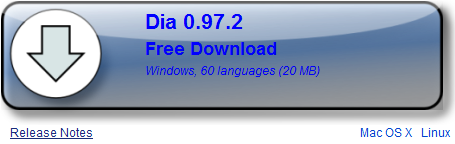
\includegraphics[scale=0.5]{images/install_01.png} 
\label{install_01}
\end{figure}
Download \'e\'en van de volgende bestanden:
\paragraph*{Ubuntu}
(\textit{http://dia-installer.de/})\ref{install_01}\linebreak
In Ubuntu is Dia ook simpelweg te installeren via het ubuntu software center.
\paragraph*{Windows}
(\textit{http://dia-installer.de/})\ref{install_01}\linebreak
De source packages zijn te downloaden van \textit{http://ftp.gnome.org/pub/gnome/sources/dia/}
\paragraph*{Mac}
(\textit{http://dia-installer.de/})\ref{install_01}\linebreak
De source packages zijn te downloaden van \textit{http://ftp.gnome.org/pub/gnome/sources/dia/}
\begin{figure}[H]
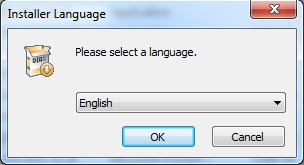
\includegraphics[scale=0.75]{images/install_02.png}
\centering
\vspace{-10pt}
\caption{Installatie van Dia : stap 1}
\label{install_02}
\end{figure}
\begin{figure}[H]
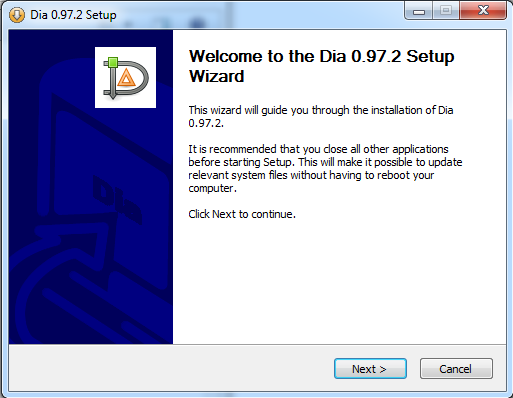
\includegraphics[scale=0.5]{images/install_03.png}
\label{install_03}
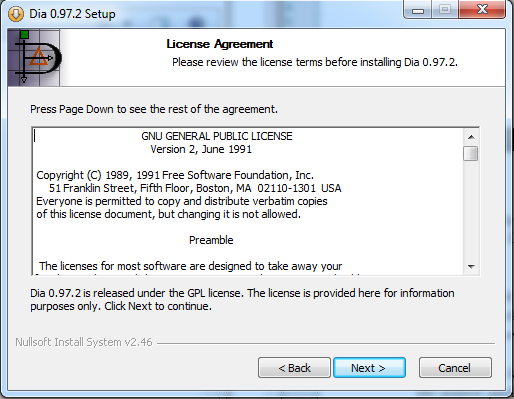
\includegraphics[scale=0.5]{images/install_04.png}
\label{install_04}
\vspace{-25pt}
\caption{Installatie van Dia : stap 2 \& 3} 
\end{figure}
\begin{figure}[H]
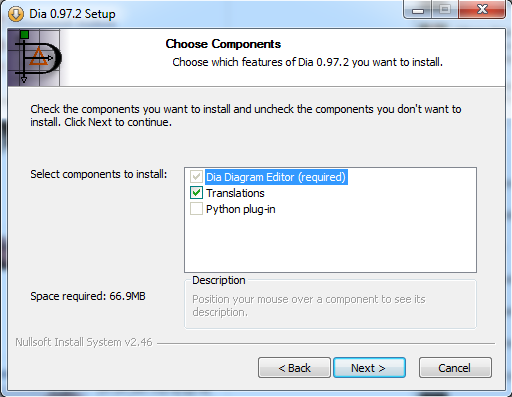
\includegraphics[scale=0.5]{images/install_05.png}
\label{install_05}
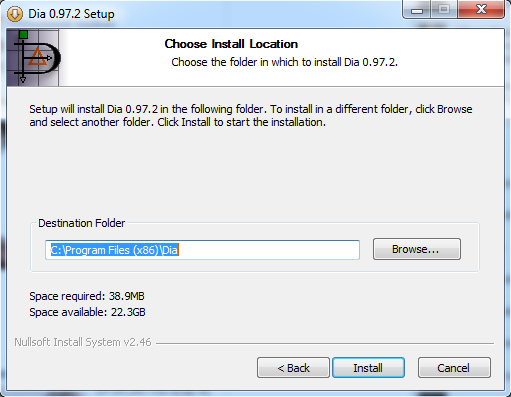
\includegraphics[scale=0.5]{images/install_06.png}
\label{install_06}
\centering 
\vspace{-25pt}
\caption{Installatie van Dia : stap 4 \& 5}  
\end{figure}
\pagebreak
%\end{}
%\begin{sectie "Gebruik van Dia"}
\section{Gebruik van Dia}
%\begin{subsectie "Aanmaken van shapes"}
\subsection{Aanmaken van shapes}
Er zijn 2 manieren om een vorm aan te maken in Dia.
\paragraph*{1}
De meest eenvoudige manier vergt geen kennis van XML of eenderwelk andere computertaal. Hierbij kan echter enkel een vorm worden gemaakt door verschillende bestaande vormen samen te voegen. Maak de gewenste vorm door verschillende vormen te slepen uit de toolbox. Ga vervolgens in het navigatiemenu bovenaan naar File/Export. Kies in het volgende venster het bestandstype Dia Shape File\index{shape file} (*.shape). In het scherm dat u nu ziet\ref{shape_01}, moet u de gewenste grootte van de vorm ingeven. 
\begin{figure}[H]
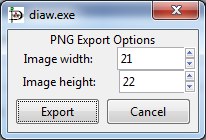
\includegraphics[scale=1]{images/shape_01.png}
\label{shape_01}
\centering
\vspace{-10pt}
\caption{nieuwe vorm : formaat instellen}
\end{figure}
Druk vervolgens op Export. De vorm is beschikbaar.
\pagebreak
\paragraph*{}
Om de vorm toe te voegen aan een diagram gaat u via het navigatiemenu naar File|Sheets and Objects. In dit vester kiest u in het linker drop-down menu de optie "Civil".\ref{shape_02}
\begin{figure}[H]
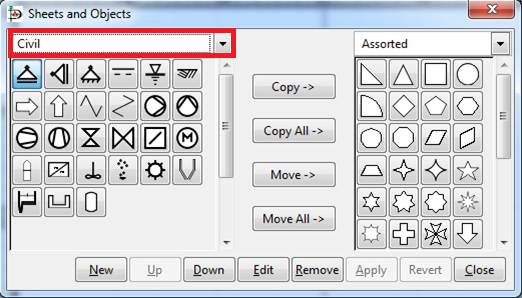
\includegraphics[scale=1]{images/shape_02.png}
\label{shape_02}
\centering
\vspace{-25pt}
\caption{nieuwe vorm : groep selecteren} 
\end{figure}
Om de vorm toe te voegen klikt u op de knop "New". In het volgende scherm moet u het pad ingeven van het .shape file. Dit doet u best via de knop "Browse".\ref{shape_03}
\begin{figure}[H]
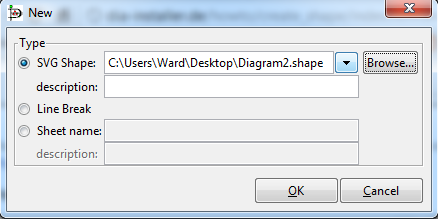
\includegraphics[scale=1]{images/shape_03.png}
\label{shape_03}
\centering
\vspace{-10pt}
\caption{nieuwe vorm : afbeelding linken} 
\end{figure}
In het tekstvak description geeft u een beschrijving van het object in. Klik op "OK" en de vorm is toegevoegd aan het Civil menu.
\paragraph*{2}
De tweede manier vergt enige kennis van XML-code. 
Maak een bestand aan met notepad, wordpad of een ander tekstbewerkingsprogramma.
Voer een reeks code in zoals in figure 1.7\ref{shape_04}.
\begin{figure}[H]
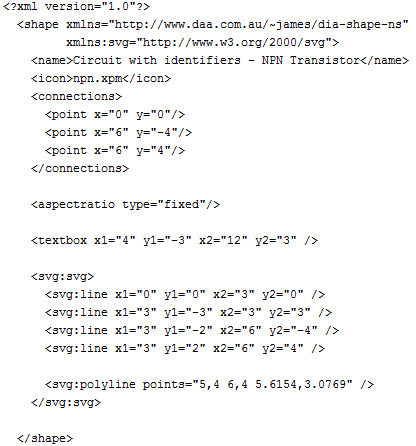
\includegraphics[scale=1]{images/shape_04.png}
\label{shape_04}
\centering 
\vspace{-10pt}
\caption{voorbeeld van XML-code voor een shape}
\end{figure}
Sla dit document op als een *.shape file. Doorloop nu de stappen van de eerste manier om de vorm toe te voegen aan Dia.
\pagebreak
%\end{}
%\begin{subsectie "Werken met Dia"}
\subsection{Werken met Dia}
%\begin{subsubsectie "Het werkveld"}
\subsubsection{Het werkveld}\ref{werkveld_01}
\begin{figure}[H]
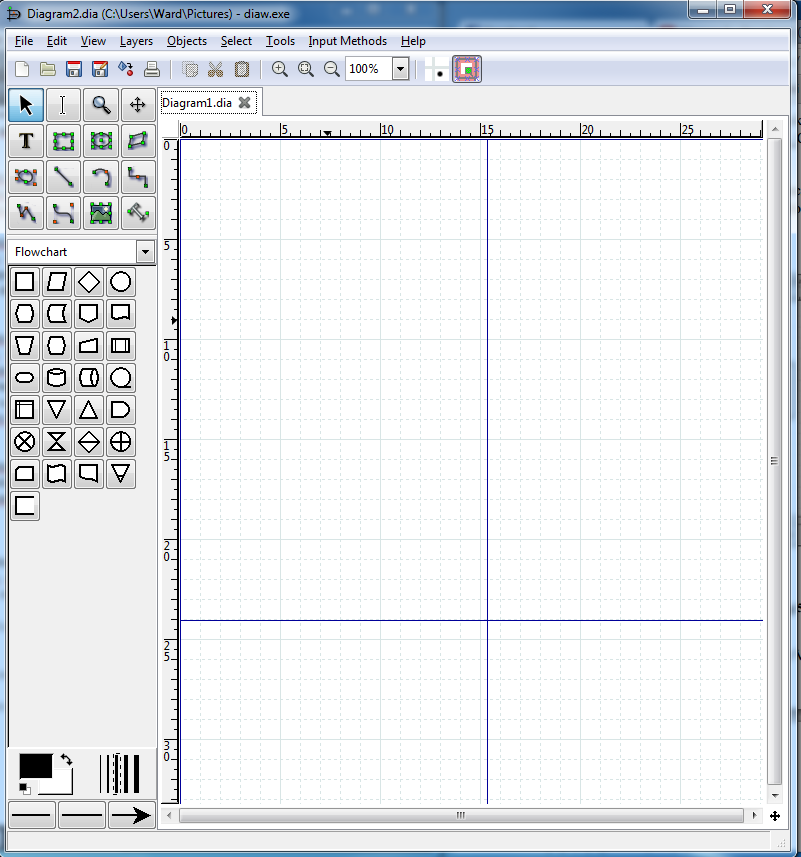
\includegraphics[scale=0.5]{images/werkveld_01.png}
\label{werkveld_01}
\centering 
\vspace{-10pt}
\caption{Het werkveld van Dia 0.97.2}
\end{figure}
\paragraph*{}
Bovenaan vindt u zoals bij elke applicatie de standaard menubalk met daaronder een menubalk van DIA zelf. Links in het venster staat de werkbalk met de diagrammen in een drop down menu zoals de afbeelding hieronder laat zien (figure 1.9)\ref{werkveld_02}. Rechts van de werkbalk bevind zich het echte werkveld waarin u het diagram zal plaatsen.
\begin{figure}[H]
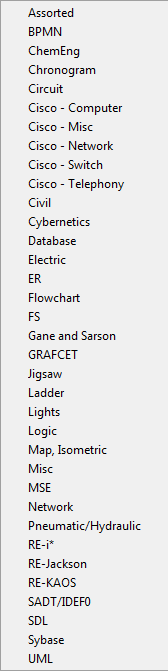
\includegraphics[scale=0.5]{images/werkveld_02.png}
\label{werkveld_02}
\centering 
\vspace{-10pt}
\caption{standaard geïmplementeerde diagramsoorten}
\end{figure}
%\end{}
%\begin{subsubsectie "Een diagram maken"}
\subsubsection{Een diagram maken}
\paragraph*{}
Een diagram maken in Dia is zeer eenvoudig aangezien alle symbolen in de werkbalk staan. U moet enkel naar het juiste item in het drop-down menu navigeren voor de juiste symbolen. Hieronder enkele voorbeelden van diagrammen, gemaakt in Dia.
\begin{enumerate}
\item	elektronisch shema\ref{voorbeeldschema_elektronisch}\index{elektronisch schema}
\item	elektrisch schema\ref{voorbeeldschema_elektrisch}\index{elektrisch schema}
\item	entity relation diagram\ref{voorbeeldschema_ERD}\index{ERD schema}
\item	logisch schema\ref{voorbeeldschema_logisch}\index{logisch schema}
\item	mindmap\ref{voorbeeldschema_mindmap}\index{mindmap}
\item	stroomdiagram\ref{voorbeeldschema_stroomdiagram}\index{stroomschema}
\end{enumerate}
\begin{figure}[H]
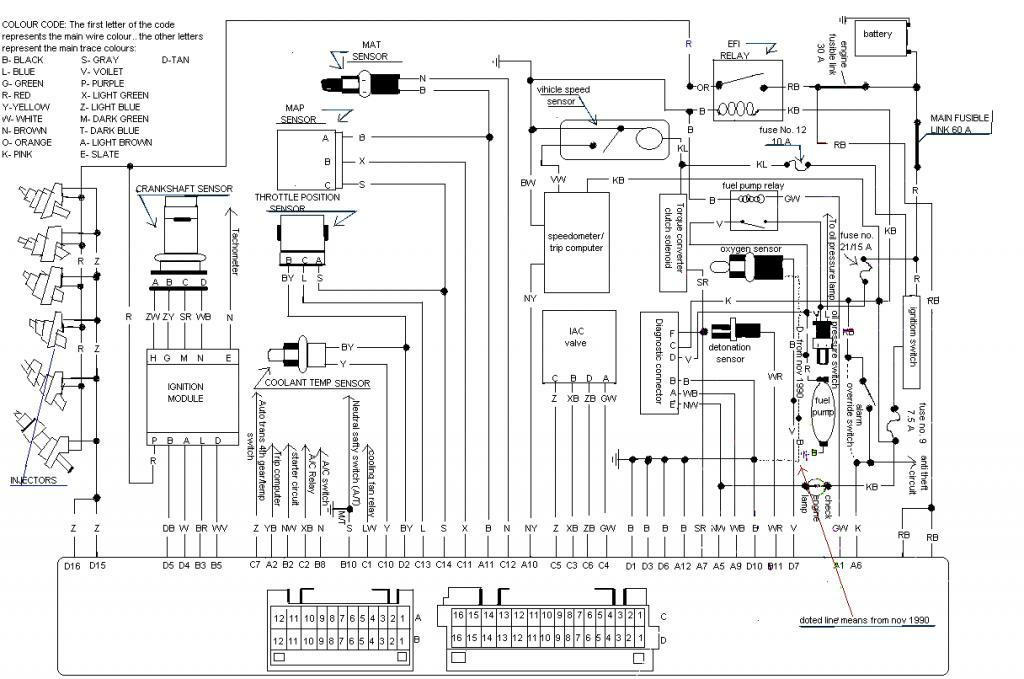
\includegraphics[scale=0.5]{images/voorbeeldschema_elektronisch.png}
\label{voorbeeldschema_elektronisch}
\centering 
\vspace{-10pt}
\caption{elektronisch schema}
\end{figure}
\begin{figure}[H]
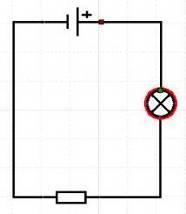
\includegraphics[scale=1]{images/voorbeeldschema_elektrisch.png}
\label{voorbeeldschema_elektrisch}
\centering 
\vspace{-10pt}
\caption{elektrisch schema}
\end{figure}
\begin{figure}[H]
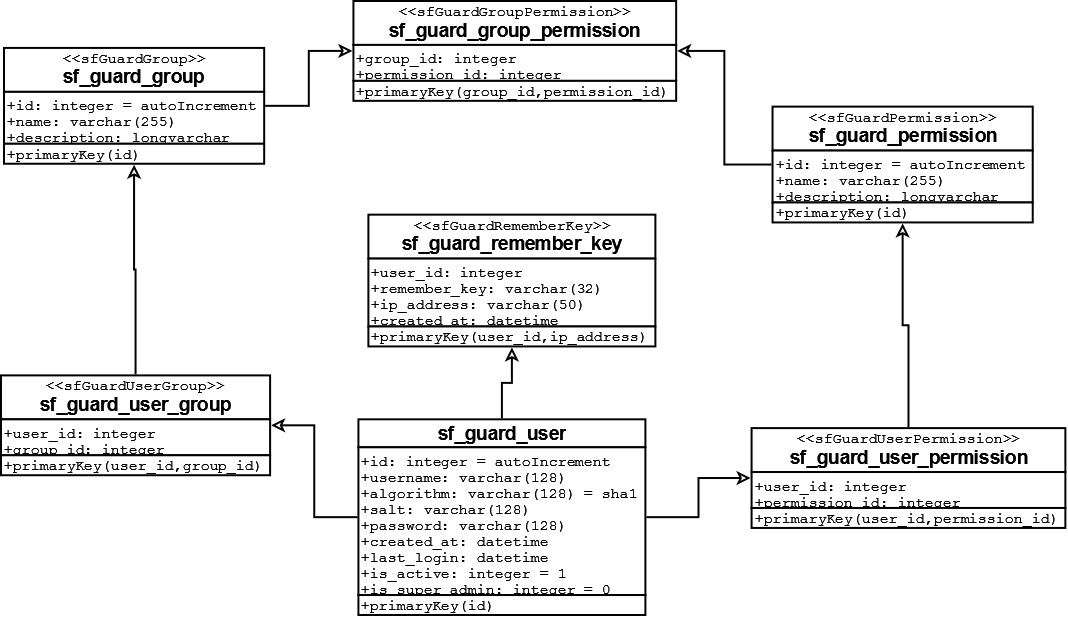
\includegraphics[scale=0.25]{images/voorbeeldschema_ERD.png}
\label{voorbeeldschema_ERD}
\centering 
\vspace{-10pt}
\caption{Entity Relation Diagram}
\end{figure}
\begin{figure}[H]
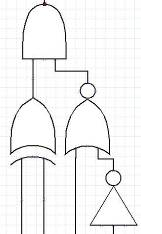
\includegraphics[scale=1]{images/voorbeeldschema_logisch.png}
\label{voorbeeldschema_logisch}
\centering 
\vspace{-10pt}
\caption{logisch schema}
\end{figure}
\begin{figure}[H]
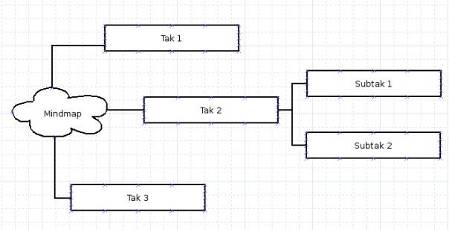
\includegraphics[scale=1]{images/voorbeeldschema_mindmap.png}
\label{voorbeeldschema_mindmap}
\centering 
\vspace{-10pt}
\caption{mindmap}
\end{figure}
\begin{figure}[H]
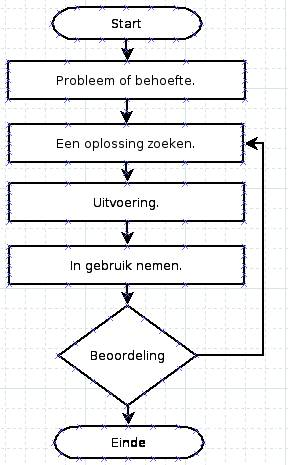
\includegraphics[scale=1]{images/voorbeeldschema_stroomdiagram.png}
\label{voorbeeldschema_stroomdiagram}
\centering 
\vspace{-10pt}
\caption{stroomdiagram}
\end{figure}
%\end{}
%\end{}
%\end{}
%\begin{sectie Concurrentie}
\section{Concurrentie}
\begin{table}
\begin{tabular}{|| l | l | l | p{3cm} ||}
\hline\hline
Naam & Creator & Open Source & Programming language used\\
\hline
\textbf{Dia} & \textbf{GNOME Office} &  \textbf{Yes} & \textbf{C}\\
StructuredViews & AgileJ & No & Java\\
UModel & Altova & No & Java,C\#,Visual basic\\
UML2 Tools & Eclipse Foundation & Yes & Java\\
MagicDraw UML & No Magic & No & Java\\
Visual Paradigm & Visual Paradigm & No & Java\\
\hline\hline
\end{tabular}
\centering
\caption{Andere UML programma's}
\end{table}
%\end{}



\chapter{Versiebeheer}
%\begin{sectie "Wat is GIT?"}
\section{Wat is GIT?}
\paragraph*{}
Voor de toepassing van versiebeheer\index{versiebeheer} is er gebruik gemaakt van het programma GIT\index{GIT}, te downloaden van http://git-scm.com/downloads.
\paragraph*{}
Git is een vrij gedistribueerd versiebeheersysteem. Het is gemaakt voor de ontwikkeling van de linuxkernel\index{linuxkernel} door Linus Torvalds. Iedere GIT werkmap bevat de volledige repository\index{repository} met een compleet historisch overzicht en volledige tracking capaciteiten. In tegenstelling tot CVS\index{CVS} of SVN\index{SVN}, concurrenten op het gebied van versiebeheer, is GIT\index{GIT} niet afhankelijk van een gemeenschappelijke locatie of een centrale server.
\paragraph*{}
In dit document is gebruik gemaakt van een repository server van GitHub\index{GitHub}, al is dit niet nodig en kan het ook locaal worden toegepast.
Op \textit{http://help.github.com/win-set-up-git/} is een zeer goede tutorial te vinden voor het installeren en gebruiken van GIT\index{GIT} en Github\index{GitHub}.
%\end{}
%\begin{sectie "Aanpassen van de github-directory"}
\section{Aanpassen van de GitHub-directory}\index{GitHub-directory}
Voor het toevoegen, bewerken of verwijderen van een bestand moeten een aantal stappen worden doorlopen.
\paragraph*{1}
Indien u een bestand wil toevoegen, moet u ervoor Zorgen dat het bestand in de directory staat die u in de tutorial heeft aangemaakt.
\paragraph*{2}
Met het commando "git status"\index{git status} zal GIT\index{GIT} zoeken naar wijzigingen in de aangeduide directory en deze tonen.
\paragraph*{3}
Om een bestand toe te voegen maakt u gebruik van het commando "git add \index{git add} \textit{NAAM VAN HET BESTAND}"\ref{git_01}, om een bestand te verwijderen is het commando "git rm \index{git rm}\emph{NAAM VAN HET BESTAND}" van toepassing.
\begin{figure}[H]
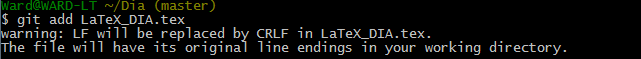
\includegraphics[scale=0.75]{images/git_01.png}
\label{git_01}
\centering 
\vspace{-10pt}
\caption{toevoegen van een bestand aan git}
\end{figure} 
\paragraph*{4}
Vervolgens moet u het bestand committen door gebruik te maken van het commando "git commit \index{git commit} -m \textit{TITEL VAN DE BEWERKING}"\ref{git_02}
\begin{figure}[H]
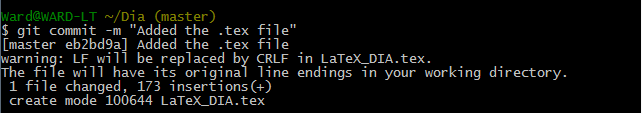
\includegraphics[scale=0.75]{images/git_02.png}
\label{git_02}
\centering 
\vspace{-10pt}
\caption{committen van bewerkingen in git}
\end{figure}  
\paragraph*{5}
Ten slotte moet de wijziging worden doorgevoerd naar de github server. Dit doet u via het commando "git push\index{git push} origin master"\ref{git_03}.
\begin{figure}[H]
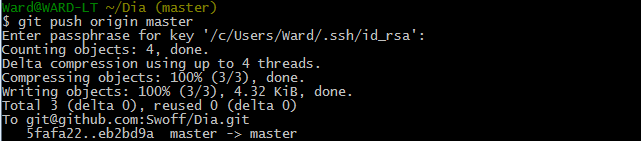
\includegraphics[scale=0.75]{images/git_03.png}
\label{git_03}
\centering 
\vspace{-10pt}
\caption{bewerkingen doorvoeren naar github}
\end{figure} 
%\end{}
\chapter{Mailserver}
%\begin{sectie Wat is Mutt?}
\section{Wat is Mutt?}
\paragraph*{}
Voor het configureren van een email-client\index{e-mail client} in linux\index{Linux} is er gebruik gemaakt van het programma Mutt\index{Mutt}, te installeren in de terminal van linux via het commando "sudo apt-get install mutt".
\paragraph*{}
Hierdoor worden mutt en postfix\index{postfix} automatisch geinstalleerd. Er wordt u gevraagd op welke manier u mutt\index{mutt} wil configureren. U kan kiezen tussen een aantal opties. In dit voorbeeld is er gekozen voor de optie "Internet site". Hierna moet u een string-waarde ingeven voor mail, vb. "wardP@linux.be"
\paragraph*{}
Verder moeten ook nog de imap-instellingen worden ingevoerd. Dit doet u door een bestand ".muttcr" aan te maken in de directory "ect" en hierin vult volgende tekst:
\begin{figure}[H]
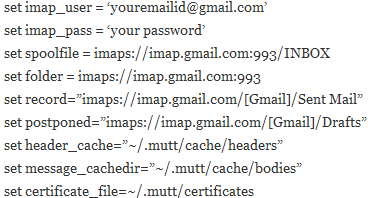
\includegraphics[scale=0.75]{images/imap_01.png}
\label{imap_01}
\centering 
\vspace{-10pt}
\caption{code configuratie imap}
\end{figure}  
\pagebreak
\paragraph*{}
Om mutt te starten voert u het commando "mutt" in in de terminal.
\begin{figure}[H]
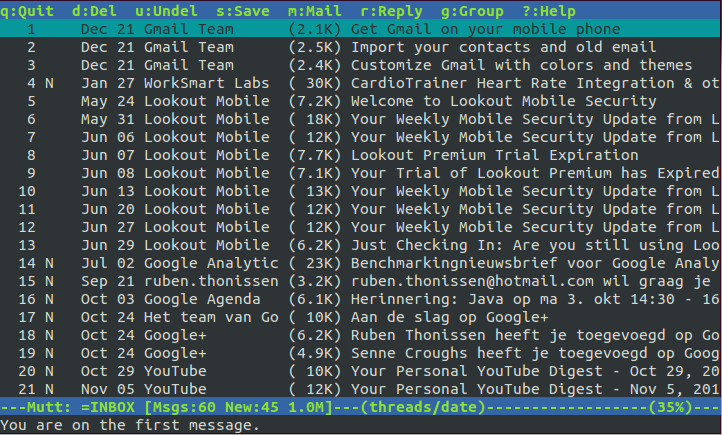
\includegraphics[scale=0.75]{images/mutt_01.png}
\label{mutt_01}
\centering 
\vspace{-10pt}
\caption{beginscherm mutt}
\end{figure} 
\pagebreak
%\begin{subsection create mail}
\section{Create mail}
\paragraph*{}
Bovenaan in het scherm van mutt staan een aantal commando's om specifieke acties uit te voeren, hierbij staat "m" voor een mail opstellen. U wordt gevraagd een email-adres van de gewenste contactpersoon in te geven en het onderwerp van de mail. Hierna krijgt u het volgende scherm te zien.
\begin{figure}[H]
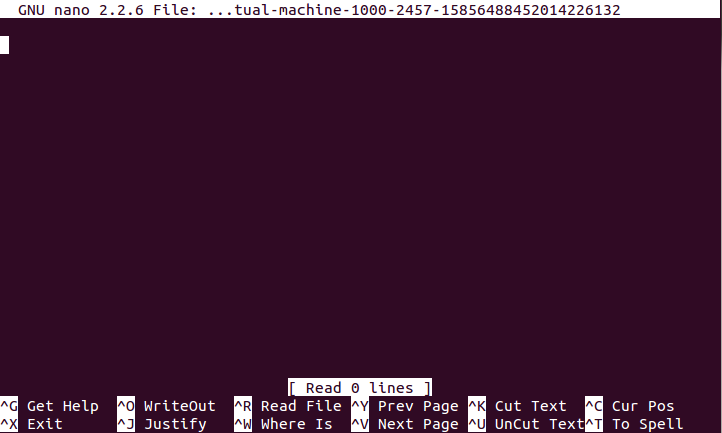
\includegraphics[scale=0.75]{images/mutt_02.png}
\label{mutt_01}
\centering 
\vspace{-10pt}
\caption{mailscherm mutt}
\end{figure}
\paragraph*{}
In dit scherm kan u de inhoud van de mail typen en opmaken via de commando's die onderaan het scherm staan. Als u de mail heeft voltooid, gebruikt u de toetsencombinatie "ctrl+O" om de mail op te slaan. Om de mail te kunnnen versturen moet u uit dit venster, dit verkrijgt u door de toetsencombinatie "ctrl+X".
\begin{figure}[H]
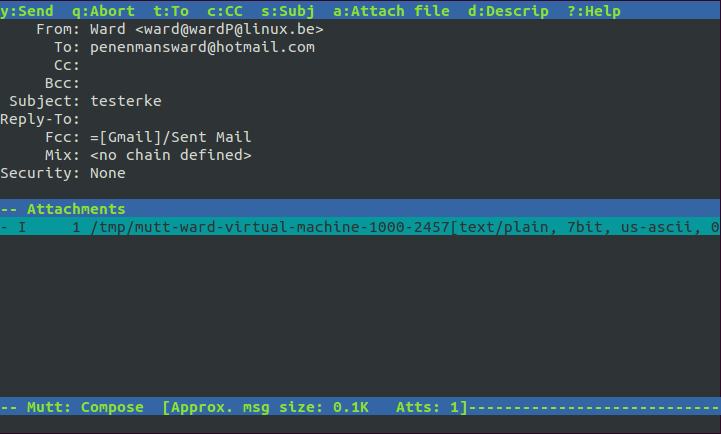
\includegraphics[scale=0.75]{images/mutt_03.png}
\label{mutt_03}
\centering 
\vspace{-10pt}
\caption{samenvatting mail mutt}
\end{figure}
\paragraph*{}
Om de mail te versturen gebruikt u het commando "y".
\subsection{Bash script}
Met het bash script\index{bash script} mailreviewer.sh (figure 3.5)\ref{bash_01} wordt dit bestand in linux\index{Linux} verstuurd naar het e-mail adres dat wordt gevraagd door het script en wordt het bestand hetnoemd naar \textit{voornaamContactpersoon.achternaamContactpersoon.pdf}
\begin{figure}[H]
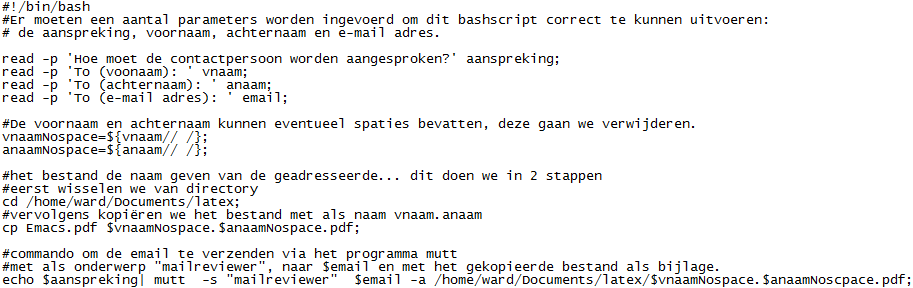
\includegraphics[scale=0.75]{images/bash_01.png}
\label{bash_01}
\centering 
\vspace{-10pt}
\caption{Bash script opdracht}
\end{figure}
%\end{}

\listoffigures
\listoftables

BibTeX ~\cite{BibTeX}.
LaTeX ~\cite{WikiBooks}.
Texmaker ~\cite{Texmaker}.
Gebruikershandleiding voor Dia ~\cite{Dia_Manual}.
Introductie van Dia ~\cite{Dia_Intro}.
Eindwerk met hoofdstuk over Dia ~\cite{Dia_Eindwerk}.
Officiele site van Dia ~\cite{Dia_Official}.

\bibliography{LaTeX_DIA}
\bibliographystyle{plain}
\printindex

\end{flushleft}
\end{document}

